%%%%%%%%%%%%%%%%%%%%%%%%%%%%% Define Article %%%%%%%%%%%%%%%%%%%%%%%%%%%%%%%%%%
\documentclass[oneside]{report}
\usepackage[svgnames,dvipsnames,x11names]{xcolor}
\RequirePackage[fontsize=14pt]{fontsize}
\linespread{1.05}
% \overfullrule=1pt
%%%%%%%%%%%%%%%%%%%%%%%%%%%%%%%%%%%%%%%%%%%%%%%%%%%%%%%%%%%%%%%%%%%%%%%%%%%%%%%
\usepackage[explicit]{titlesec}
\usepackage{graphicx} % Required for inserting images
\usepackage{varwidth}
\usepackage{tikz}
\usetikzlibrary{calc,shadows,hobby,intersections, decorations.markings, decorations.pathreplacing,spy,arrows,shapes,fadings,trees,mindmap,patterns,shapes.arrows,shapes.symbols,tikzmark,shapes.geometric,graphs, quotes, angles,decorations.pathmorphing,through,shadings,backgrounds,positioning,fit,arrows.meta,shapes.misc,decorations.shapes}
\pgfdeclarelayer{background} %背景%底层
\pgfdeclarelayer{foreground} %上层
\pgfdeclarelayer{top} %顶部
\pgfdeclarelayer{bottom} %底部
\pgfsetlayers{bottom,background,main,foreground,top}
\tikzfading[name=fade right,
                    right color =transparent!100,
                    left color=transparent!50]
\tikzfading[name=fade left,
                    left color =transparent!100,
                    right color=transparent!50]
\tikzfading[name=fade up,
                    top color =transparent!30,
                    bottom color=transparent!0]
\tikzfading[name=fade down,
                    bottom color =transparent!100,
                    top color=transparent!50]
%% -------- 章节样式
\definecolor{gray1}{HTML}{9E9E9E}
\definecolor{gray2}{HTML}{d4d3d8}
\definecolor{black1}{HTML}{616065}

\newcommand{\chapternumbered}[1]{%
    \begin{tikzpicture}[remember picture,overlay]
    \def\xshiftofnode{2cm}
    \def\hlenofnode{2.8cm}
    \def\vlenofnode{4.76cm}
    \def\nodecorners{8pt}
    \def\chapnameyshift{0.7cm}
    \def\chapbackheightI{.1\paperheight}
    \def\chapbackheightII{.15\paperheight}
        \fill[gray2] % 浅色
        (current page.north west) coordinate (NW) --++(0,-\chapbackheightII) [bend left=-9] to ([shift={(\paperwidth,-.8*\chapbackheightI-2.96cm)}]NW) |- (NW)  --cycle; % bottom background
        \fill[gray1!80] % 深色
        (current page.north west) coordinate (NW) --++(0,-\chapbackheightI) [bend left=-10] to ([shift={(\paperwidth,-.8*\chapbackheightI-3.5cm)}]NW) |- (NW)  --cycle; % subbottom background
        %%%%%%%%%%%%%%%%%% Chapname Box %%%%%%%%%%%%%%%%%%%%
        \fill[black1,opacity=0.8]
            ([xshift=\xshiftofnode]NW) {[rounded corners=\nodecorners]--++(0,-\vlenofnode)} coordinate (chapnameleft) {[rounded corners=\nodecorners]--++(\hlenofnode,0)} coordinate (chapnameright) --++(0,\vlenofnode)--cycle;
        \pattern[pattern=sixpointed stars,pattern color=gray2!50,opacity=0.8]
            ([xshift=\xshiftofnode]NW)--++(0,-0.76*\vlenofnode) coordinate (bendl) [bend left=-2] to  ([shift={(\hlenofnode,-0.168*\vlenofnode)}]bendl) |- ([xshift=\xshiftofnode]NW) --cycle;
        \fill [black1,path fading=fade up]%
            ([xshift=\xshiftofnode]NW)--++(0,-0.76*\vlenofnode) coordinate (bendl) [bend left=-2] to  ([shift={(\hlenofnode,-0.168*\vlenofnode)}]bendl) |- ([xshift=\xshiftofnode]NW) --cycle;
        %%%%%%%%%%%%%%%%%% Chapname Box %%%%%%%%%%%%%%%%%%%%
        \node[font=\huge\bfseries,text=gray!20!white] (chapname) at ($([yshift=\chapnameyshift]chapnameleft)!0.5!([yshift=\chapnameyshift]chapnameright)$) {CH\ \thechapter}; %chapname
        \node[above right,font=\huge\bfseries,text=black] (chaptitle) at ([shift={(1.5cm,-1.2*\chapnameyshift)}]chapname) {\begin{varwidth}{.92\linewidth} \baselineskip=23pt #1\end{varwidth}}; % chaptitle
    \end{tikzpicture}
}
\newcommand{\chapternonum}[1]{%
    \begin{tikzpicture}[remember picture,overlay]
    \def\xshiftofnode{2cm}
    \def\hlenofnode{2.8cm}
    \def\vlenofnode{4.76cm}
    \def\nodecorners{8pt}
    \def\chapnameyshift{0.6cm}
    \def\chapbackheightI{.1\paperheight}
    \def\chapbackheightII{.15\paperheight}
        \fill[gray2]
        (current page.north west) coordinate (NW) --++(0,-\chapbackheightII) [bend left=-9] to ([shift={(\paperwidth,-.8*\chapbackheightI-2.96cm)}]NW) |- (NW)  --cycle; % bottom background
        \fill[gray1!80]
        (current page.north west) coordinate (NW) --++(0,-\chapbackheightI) [bend left=-10] to ([shift={(\paperwidth,-.8*\chapbackheightI-3.5cm)}]NW) |- (NW)  --cycle; % subbottom background
        %%%%%%%%%%%%%%%%%% Chapname Box %%%%%%%%%%%%%%%%%%%%
        \fill[black1,opacity=0.8]
            ([xshift=\xshiftofnode]NW) {[rounded corners=\nodecorners]--++(0,-\vlenofnode)} coordinate (chapnameleft) {[rounded corners=\nodecorners]--++(\hlenofnode,0)} coordinate (chapnameright) --++(0,\vlenofnode)--cycle;
        \pattern[pattern=sixpointed stars,pattern color=gray2!50,opacity=0.8]
            ([xshift=\xshiftofnode]NW)--++(0,-0.76*\vlenofnode) coordinate (bendl) [bend left=-2] to  ([shift={(\hlenofnode,-0.168*\vlenofnode)}]bendl) |- ([xshift=\xshiftofnode]NW) --cycle;
        \fill [black1,path fading=fade up]%
            ([xshift=\xshiftofnode]NW)--++(0,-0.76*\vlenofnode) coordinate (bendl) [bend left=-2] to  ([shift={(\hlenofnode,-0.168*\vlenofnode)}]bendl) |- ([xshift=\xshiftofnode]NW) --cycle;
        %%%%%%%%%%%%%%%%%% Chapname Box %%%%%%%%%%%%%%%%%%%%
        \node[font=\fontsize{30pt}{30pt}\selectfont\scshape,text=gray!20!white] (chapname) at ($([yshift=\chapnameyshift]chapnameleft)!0.5!([yshift=\chapnameyshift]chapnameright)$) {chap}; %chapname
        \node[right,font=\huge\bfseries,text=black] (chaptitle) at ([shift={(1.5cm,0)}]chapname) {\begin{varwidth}{.92\linewidth} \baselineskip=23pt #1\end{varwidth}}; % chaptitle
    \end{tikzpicture}
}

\titleformat{\chapter}{\huge\bfseries}{}{1em}{\chapternumbered{#1}}
\titleformat{name=\chapter,numberless}{\bfseries\huge}{}{1em}{\chapternonum{#1}}
\titlespacing{\chapter}{0pt}{0pt}{65pt}
%%%%%%%%%%%%%%%%%%%%%%%%%%%%% Using Packages %%%%%%%%%%%%%%%%%%%%%%%%%%%%%%%%%%
\usepackage{geometry}
\usepackage{amssymb}
\usepackage{hyperref}
\usepackage{amsmath}
\usepackage{amsthm}
\usepackage{empheq}
\usepackage{mdframed}
\usepackage{booktabs}
\usepackage{lipsum}
\pagecolor{gray!15}
\usepackage{psfrag}
\usepackage{bbding}
\usepackage{fancyhdr}
\makeatletter
\fancypagestyle{main}{
    \fancyhf{}
    % \renewcommand{\headrulewidth}{0pt}
    \fancyhead[C]{\fontsize{13pt}{13pt}\selectfont\sc\@title}
    \fancyfoot[C]{\normalsize\thepage}
}
\makeatother
\usepackage{enumitem}
\setlist{parsep=5pt,itemsep=5pt,font=\upshape} % 取消所有列表默认距离
\usepackage{pgfplots}
% \usepackage{bm}
\usepackage{stix}
\usepackage{bropd,physics}
\usepackage{indentfirst}
\usepackage{float}
\usepackage{pifont}
\usepackage{pgfornament-han}
%%%%%%%%%%%%%%%%%%%%%%%%%%%%%%%%%%%%%%%%%%%%%%%%%%%%%%%%%%%%%%%%%%%%%%%%%%%%%%%

% Other Settings

%%%%%%%%%%%%%%%%%%%%%%%%%% Page Setting %%%%%%%%%%%%%%%%%%%%%%%%%%%%%%%%%%%%%%%
\geometry{a4paper,margin=2.2cm}
\hypersetup{
colorlinks=true,
linkcolor=black,
citecolor=purple,
}
\setlength{\headheight}{13.0pt}
%%%%%%%%%%%%%%%%%%%%%%%%%% Define some useful colors %%%%%%%%%%%%%%%%%%%%%%%%%%
\definecolor{ocre}{RGB}{243,102,25}
\definecolor{mygray}{RGB}{243,243,244}
\definecolor{deepGreen}{HTML}{a71930}
\definecolor{shallowGreen}{HTML}{f8dfc2}
\definecolor{deepBlue}{HTML}{005670}
\definecolor{shallowBlue}{HTML}{ced7df}
%%%%%%%%%%%%%%%%%%%%%%%%%%%%%%%%%%%%%%%%%%%%%%%%%%%%%%%%%%%%%%%%%%%%%%%%%%%%%%%

%%%%%%%%%%%%%%%%%%%%%%%%%% Define an orangebox command %%%%%%%%%%%%%%%%%%%%%%%%
\newcommand\orangebox[1]{\fcolorbox{ocre}{mygray}{\hspace{1em}#1\hspace{1em}}}
\newenvironment{note}[1][\bf Note:]{\Line\uuline{#1} }{\Line}
\newcommand{\Line}{\noindent\\\tikz\draw[line width=0.65pt,gray!80,dashed] (0,0)--++(.99\linewidth,0);\par}
\newcommand{\prob}[2][Problems]{\begin{center}
    \pgfornamenthan[color=#2,scale=0.25,symmetry=c]{68}\hspace{.3em}\begin{tabular}{c}  \pgfornamenthan[color=#2,scale=0.4]{60}\\[1.6em]
         \textbf{\color{#2}\fontsize{25pt}{25pt}\selectfont \textsc{#1}}  \end{tabular}\hspace{.5em}\pgfornamenthan[color=#2,scale=0.25,symmetry=h]{68}
\end{center}}
%%%%%%%%%%%%%%%%%%%%%%%%%%%%%%%%%%%%%%%%%%%%%%%%%%%%%%%%%%%%%%%%%%%%%%%%%%%%%%%

%%%%%%%%%%%%%%%%%%%%%%%%%%%% English Environments %%%%%%%%%%%%%%%%%%%%%%%%%%%%%
\newtheoremstyle{mytheoremstyle}{3pt}{3pt}{\normalfont}{0cm}{\rmfamily\bfseries}{}{.5em}{{\color{black}\thmname{#1}~\thmnumber{#2}}\thmnote{\,--\,#3}}
\newtheoremstyle{myproblemstyle}{3pt}{3pt}{\normalfont}{0cm}{\rmfamily\bfseries}{}{.5em}{{\color{black}\thmname{#1}~\thmnumber{#2}}\thmnote{\,--\,#3}}
\theoremstyle{mytheoremstyle}
\newmdtheoremenv[linewidth=3pt,backgroundcolor=deepGreen!12,linecolor=deepGreen,leftline = true,rightline=false,topline=false,bottomline=false,leftmargin=0pt,innerleftmargin=5pt,innerrightmargin=5pt,innertopmargin=3pt]{theorem}{Theorem}[section]
\theoremstyle{mytheoremstyle}
\newmdtheoremenv[linewidth=3pt,backgroundcolor=shallowBlue!70,linecolor=deepBlue,leftline = true,rightline=false,topline=false,bottomline=false,leftmargin=0pt,innerleftmargin=5pt,innerrightmargin=5pt,innertopmargin=3pt]{definition}{Definition}[section]
\theoremstyle{myproblemstyle}
\newmdtheoremenv[linecolor=black!60,backgroundcolor=gray!20,linewidth=3pt,leftline = true,rightline=false,topline=false,bottomline=false,leftmargin=0pt,innerleftmargin=5pt,innerrightmargin=5pt,innertopmargin=5pt,innerbottommargin=5pt]{problem}{Problem}[section]
\newenvironment*{solution}{\begin{proof}[SOLUTION]}{\end{proof}}
%%%%%%%%%%%%%%%%%%%%%%%%%%%%%%%%%%%%%%%%%%%%%%%%%%%%%%%%%%%%%%%%%%%%%%%%%%%%%%%

%%%%%%%%%%%%%%%%%%%%%%%%%%%%%%% Plotting Settings %%%%%%%%%%%%%%%%%%%%%%%%%%%%%
\usepgfplotslibrary{colorbrewer}
\pgfplotsset{width=8cm,compat=1.9}
%%%%%%%%%%%%%%%%%%%%%%%%%%%%%%%%%%%%%%%%%%%%%%%%%%%%%%%%%%%%%%%%%%%%%%%%%%%%%%%

%%%%%%%%%%%%%%%%%%%%%%%%%%%%%%% Title & Author %%%%%%%%%%%%%%%%%%%%%%%%%%%%%%%%
\title{Lecture Note for Topology}
%%%%%%%%%%%%%%%%%%%%%%%%%%%%%%%%%%%%%%%%%%%%%%%%%%%%%%%%%%%%%%%%%%%%%%%%%%%%%%%
\usepackage[firstpage=true]{background}
\backgroundsetup{scale=1.5,angle=0,opacity=0.3,contents={\includegraphics[width=\paperwidth, height=\paperwidth, keepaspectratio]{pexels-todd-trapani-1198828 (1).jpg}}}
\begin{document}
    \begin{titlepage}
\vspace*{\stretch{1}}
\begin{center}
  {\huge\bfseries Lecture Note for Topology  
                  }                  \\[6.5ex]
  {\large\bfseries Ethan Lu}           \\
  \vspace{4ex}
  \vspace{5pt}
  %                    \\[5pt]
  \textit{Guangxi University for Nationalities}                \\[2cm]
  Mathematics is the queen of science. \\[2cm]
  \textsc{\Large Master of Comaplex Geometry}    \\[2ex]
  \textsc{\large Mathematics}             \\[12ex]
  \vfill
  Department of Mathematics and Physics              \\
  Nanning China                                 \\
  \vfill
  \today
\end{center}
\vspace{\stretch{2}}
\end{titlepage}
    \tableofcontents
    \pagestyle{main}
    \chapter{Topology}
    \section{Topics}
    \begin{enumerate}
        \item \emph{An important fact is that a topological space is a $T_1$--space iff every point is closed.}
        \item \textit{The intersection of connected sets may not be connected!} 
        
        An illustrative instance is the set of intersection points between two curves, which comprises a finite and discrete space. It is  non-connected.
        \item 
        The key trait of a compact space $A$ is that if $\{\bigcup U_i\}$ is an open cover for $A$, then there must exist a \emph{finite open subcover} $\{\bigcup_{j\in I}U_j\}$, where $I$ is a finite index set.
        \item The union and intersection operations of topological spaces remain compact.
        \item The product space is Hausdorff ($T_2$) and path-connected, which is consistent with the generators.
        \item !!! Let $C$ be a closed and bounded subset of a metric space $(X,d)$, where we give $X$ its metric topology. \emph{Sometimes $C$ is not always compact.} 
        
        For instance, if $X$ is an infinite set with the metric $d$ where $\dd(x_1,x_2)$ is $1$ if $x_1\neq x_2$ and $0$ if $x_1=x_2$. Then $X$ is bounded and closed but only finite subsets of $X$ are compact. In particular, $X$ is closed and bounded but not compact.
        \item Let $f\colon X\to Y$ be a continuous surjective map of topological spaces such that $X$ is Hausdorff. Then $Y$ is not Hausdorff.

        Take an instance. Let $X=Y$ be any set with at least two points but give $X$ the discrete topology and give $Y$ the indiscrete topology. Let $f(x)=x$ for all $x\in X$. Then $f$ is continous , $X$ is a $T_2$--space but $Y$ is not a $T_2$--space.
        \item When prove the \emph{connectedness} of a space, we use \textit{proof by contradiction} in general. In fact, we can always assume that $X$ is disconnected, then there must exist two non-empty disjoint ($U\cap V=\emptyset$) open sets $U$ and $V$ such that $U\cup V=X$.
        \item Every path-connected space is connected space, but the converse is not true.
    \end{enumerate}
    \begin{problem}
        Let $(X,\tau)$ be a topological space. Then the following statements are equivalent.
        \begin{enumerate}[label=(\roman*)]
            \item $X$ is $T_1$--space,
            \item Each singleton subset of $X$ is closed,
            \item Each subset $A$ of $X$ is the intersection of its open supersets.
        \end{enumerate}
    \end{problem}
\begin{proof}
    \textit{(i)$\to$(ii):\quad} Let $x\in X$ and $X$ is $T_1$--space. Then for any $y\in X$ and $y\neq x$, there exists a neighborhood $V$ of $y$ such that $x\not\in V$, i.e. $V\cap \{x\}=\emptyset$. Thus, $y\not\in \overline{\{x\}}$, then $\{x\}=\overline{\{x\}}$. (Here, we use the fact that $y\not\in \{x\}^d$ for $V\cap (\{x\}-\{y\})=V\cap \{x\}$. It is clear that $y\not\in\{x\}$ and $\overline{\{x\}}=\{x\}\cup \{x\}^d$.) Then $\{x\}$ is closed.
    \Line
    \textit{(ii)$\to$(i):\quad} Let $\{x\}$ be closed for any $x\in X$. Then for any $y\in X$ and $y\neq x$, one abtains that $y\not\in \{x\}=\overline{\{x\}}$. It suffices to show that $y\in \{x\}^c$, which means that $X$ is $T_1$--space.
    \Line
    \textit{(ii)$\to$(iii):\quad} Suppose any singleton subset of $X$ is closed and let $A\subseteq X$. We can write 
    \[A=\bigcup_{x\in A} \{x\}.\]
    Let $y\in X$ and $y\not\in A$, then $y\neq x$. By assumption, $\{y\}$ is closed. Thus $\{y\}^c$ is open. As $A\subseteq \{y\}^c$ for any $y\not\in A$, thus $A=\bigcap_{y\not\in A}\{y\}^c$, i.e. $A$ is the intersection of its open supersets.
    \Line
    \textit{(iii)$\to$(i):\quad} According to the above, one has $A=\bigcap_{y\not\in A}\{y\}^c$, where $A\subseteq\{y\}^c$. For any $x\in A$, we gain $x\in \{y\}^c$ and $y\not\in A$ i.e. $y\neq x$, which suffice to show that $X$ is $T_1$--space.
\end{proof}
\begin{problem}
    An infinite set with \textbf{co-finite topology} is $T_1$ but not $T_2$.
\end{problem}
\begin{proof}
    Suppose the contrary is true, i.e. $X$ is $T_2$. Then for any $a,b\in X$, there are two open subsets $U,V$ such that $a\in U$, $b\in V$ and $U\cap V=\emptyset$.

    \[{\color{NavyBlue} U^c\cup V^c}=(U\cap V)^c {\color{purple}= }  \emptyset^c={\color{MediumVioletRed}X}\]
    The left hand side is the union of two finite sets, but the right hand side is an infinite set $X$, which is a contradiction. Thus $X$ is not $T_2$.
\end{proof}


\paragraph{Regular Space}
\begin{figure}[H]
    \centering
\tikzset{every picture/.style={line width=0.75pt}} %set default line width to 0.75pt        

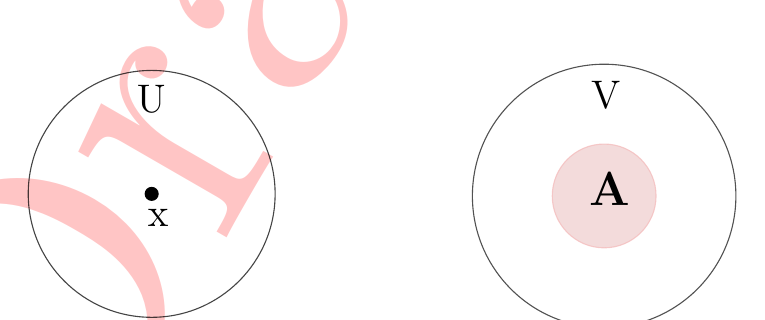
\begin{tikzpicture}[x=0.75pt,y=0.75pt,yscale=-1,xscale=1]
%uncomment if require: \path (0,300); %set diagram left start at 0, and has height of 300

%Shape: Circle [id:dp9756628765848725] 
\draw  [color={rgb, 255:red, 0; green, 0; blue, 0 }  ,draw opacity=0.73 ] (132.05,161.47) .. controls (132.05,128.63) and (158.68,102) .. (191.53,102) .. controls (224.37,102) and (251,128.63) .. (251,161.47) .. controls (251,194.32) and (224.37,220.95) .. (191.53,220.95) .. controls (158.68,220.95) and (132.05,194.32) .. (132.05,161.47) -- cycle ;
%Shape: Circle [id:dp0020769997121046213] 
\draw  [color={rgb, 255:red, 0; green, 0; blue, 0 }  ,draw opacity=0.68 ] (346.05,162.47) .. controls (346.05,127.42) and (374.47,99) .. (409.53,99) .. controls (444.58,99) and (473,127.42) .. (473,162.47) .. controls (473,197.53) and (444.58,225.95) .. (409.53,225.95) .. controls (374.47,225.95) and (346.05,197.53) .. (346.05,162.47) -- cycle ;
%Shape: Circle [id:dp11826540106467331] 
\draw  [color={rgb, 255:red, 244; green, 187; blue, 187 }  ,draw opacity=0.75 ][fill={rgb, 255:red, 233; green, 189; blue, 189 }  ,fill opacity=0.55 ] (384.53,162.47) .. controls (384.53,148.67) and (395.72,137.47) .. (409.53,137.47) .. controls (423.33,137.47) and (434.53,148.67) .. (434.53,162.47) .. controls (434.53,176.28) and (423.33,187.47) .. (409.53,187.47) .. controls (395.72,187.47) and (384.53,176.28) .. (384.53,162.47) -- cycle ;
%Shape: Circle [id:dp6696414603049186] 
\draw  [fill={rgb, 255:red, 0; green, 0; blue, 0 }  ,fill opacity=1 ] (188.41,161.47) .. controls (188.41,159.75) and (189.8,158.36) .. (191.53,158.36) .. controls (193.25,158.36) and (194.64,159.75) .. (194.64,161.47) .. controls (194.64,163.2) and (193.25,164.59) .. (191.53,164.59) .. controls (189.8,164.59) and (188.41,163.2) .. (188.41,161.47) -- cycle ;

% Text Node
\draw (401,150) node [anchor=north west][inner sep=0.75pt]   [align=left] {\textbf{{\large A}}};
% Text Node
\draw (183,108) node [anchor=north west][inner sep=0.75pt]   [align=left] {U};
% Text Node
\draw (402,106) node [anchor=north west][inner sep=0.75pt]   [align=left] {V};
% Text Node
\draw (188.41,167.47) node [anchor=north west][inner sep=0.75pt]   [align=left] {x};

\end{tikzpicture}
    \caption{(Regular Space)}
    \label{fig:regular space}
\end{figure}
A regular $T_1$--space is $T_3$--space.

\begin{problem}
    Every path-connected space is connected.
\end{problem}
\begin{proof}
    (Proof by contradiction.) Assume that a path-connected space $X$ is disconnected. Then there exist two non-empty disjoint subsets $U$ and $V$ in $X$ such that $U\cup V=X$.

    For $X$ is path-connected, there exist a continous function $f\colon [0,1]\to X$ with $f(0)=a,f(1)=b, \forall a,b\in X$. Then $f^{-1}(U)$ and $f^{-1}(V)$ are two non-empty disjoint open subsets in $[0,1]$ such that 
    \[[0,1]=f^{-1}(U)\bigcup f^{-1}(V),\]
    i.e. $[0,1]$ is dis-connected.
    It is contradictive with the fact that $[0,1]$ is connected. So $X$ is connected.
    
\end{proof}

\prob{DarkGoldenrod4}
\begin{enumerate}
    \item Any metrizable space is second-countable.\cite{kelley2017general}

    Take a discrete uncountable space. It's metrizable (for instance, with the metric where all distances $d(x,y)=1$ for $x\neq y$) but not second-countabale.
    \item Countable union of path-connected space is path-connected.
    \item Is \emph{any dense subset of the Cantor set is uncountable}? That's wrong, for instance, we take the union of boundary points of all the inetrvals in $[0,1]$ that we're using to define $C$.
    \item Be aware of the identity mapping between $X$ equipped with one topology and $X$ equipped with another topology! Because for $\mathbb{R}$, the \emph{lower limit topology} is finer than the \emph{standard topology}, and for \emph{product space}, the \emph{box topology} is finer than the \emph{product topology}.
    \item \textit{connectedness} : If topological space $X$ admits nontrival partition into open sets.
    
    \textit{compact} : If every open cover possesses a finite subcover.
    \item The \emph{diameter} of a subset $A$ of a metric space $(X,d)$ is $\sup \{d(x,y)\mid (x,y)\in A\times A\}$ .
    \item  The \emph{torus} is an orientable surface and it can be embedded without self-intersection into $\mathbb{R}^3$. The Klein bottle is a non-orientable surface which cannot be embedded without self-intersection into $\mathbb{R}^3$.
    \item Given any topological space $X$, one abtains another topological space $\mathcal{C}(X)$ with complement topology? 
    
    That's wrong! For example, 
    \item There are topological spaces with countably many points, which have uncountably many open sets?  $\surd$
    
    That's true. For example, \textit{countable set with the discrete topology}.
    \item The number of points of a finite Hausdorff space is always a \textit{prime power}? 
    
    That's wrong! For instance, \emph{$6$ -element set with the discrete topology}. (Note that \emph{finite discrete topological space is always Hausdorff.}) This is a Hausdorff space whose number of points is not a prime power.
    \item $\mathbb{R}$ with the Zariski topology is a compact topological space? $\surd$
    
    That's true! \emph{proof} : 
    \item $\mathbb{R}$ with the Zariski topology is a connected topological space?  $\surd$
    
    That's true! \emph{No subset of $\mathbb{R}$ is both finite and has a finite complement-so the above holds here.}
    \item Let $\mathbb{Z}$ be endowed with the topology where \emph{the open sets are the unions of residue classes}. Then $f\colon \mathbb{Z}\to\mathbb{Z}, n\mapsto n+(-1)^{n}$ is an homeomorphism? $\surd$
    
    The function $f$ maps uions of residue classes to unions of residue classes, so it is an homeomorphism.
\end{enumerate}

\begin{problem}
If $\{A_i : i\in N\}$ is a collection of path-connected subsets of a space $(X,\tau)$, and $\bigcap_{i\in N}A_i\neq \emptyset$ (There is atleast one common point!)
then $A=\bigcup_{i\in N}A_i$ is path-connected. In other words, countable union of path-connected sets is path-connected.
\end{problem}
\begin{proof}
    Let $x,y\in A$, where $x\in A_{i_1}, y\in A_{i_2}$. Let $z\in \bigcap_{i\in N}A_i$, then $z\in A_{i_1}, z\in A_{i_2}$.

    For $A_{i_1}$ is path-connected, there exists a continuous function $f\colon [0,1]\to A_{i_1}$ that maps $x$ to $z$ with $f(0)=x,f(1)=z$. Similarily, 
    there exists another continuous function $g\colon [0,1]\to A_{i_2}$ that maps $y$ to $z$ with $g(0)=y, g(1)=z$.

    Define function $h$ by 
    \[
        h(t)=\begin{cases}
            f(2t), & 0\leqslant t <\frac 12,\\ 
            g(2t-1), & \frac 12 \leqslant t \leqslant 1.
        \end{cases}
    \]
    Then $h$ is continuous. Thus $A$ is path-connected.
\end{proof}
\begin{problem}[$(\star\star\star)$]
     Let $\mathbb{R}^2$ be endowed with the usual topology. Either prove or disprove that $[0,1[\times ]0,1[$ and $[0,1[\times [0,1]$ are homeomorphic subspaces of $\mathbb{R}^2$.
\end{problem}

\begin{proof}

\end{proof}








\bibliography{ref}
\bibliographystyle{plain}
\end{document}
